\chapter{Introdução} \label{ch:intro}

% Resumo opcional. Comentar se não usar.
%\resumodocapitulo{Resumo opcional}

% "I never think of the future - it comes soon enough." - Albert Einstein

\section{Contextualização}


Toda tecnologia surge no intento de reduzir o gasto de energia na execução de alguma tarefa. Nela consolidamos todo o conhecimento envolvido em alguma técnica permitindo a execução com um esforço muito menor a partir da consolidação disto em um objeto. A este damos diversos nomes: ferramentas, máquinas, robôs, lápis e caneta. Essencialmente todos com a mesma missão de permitir realizar qualquer tarefa a menor quantidade de energia possível.

As primeiras tecnologias pegavam um pouco desta capacidade de executar as tarefas a partir de fenômenos naturais. Desta forma, o conhecimento aliado a propagação de calor do fogo, a fluidez da água e do vento e a rigidez da pedras nos permitiram conceber ferramentas cada vez mais complexas. Com o passar da história alcançamos o ponto dos próprios engenhos poderem ser iniciados e deixados a executarem tarefas sozinhos sem qualquer interferência de pessoas. No que então começamos a chamada automação.

% Citar alguma referência de história?
% Comentar um pouco sobre a história da automação
% História da robótica

%Dentre este universo novo de máquinas surge então o robô na tentativa replicar as capacidades humanas originadas em meio a evolução em um engenho que pude-se ser replicado e controlado. Em particular, replicar a capacidade de interagir com objetos de uma forma mais livre sem a necessidade de um completo estudo a respeito.

Robôs industriais, ou manipuladores robóticos, como também são chamados, se tornaram parte essencial na produção de bens aonde alguma das etapas exijam capacidades sobre-humanas de força, precisão, repetibilidade ou ainda na tolerância a altas temperatura e materiais corrosivos. Garantindo assim consistência, rapidez e segurança em tarefas de soldagem, montagem, pintura e corte no cenário industrial. No entanto, estas mesmas características que conferem a robustez apreciada no ambiente industrial tornam os robôs perigosos. A força, peso e velocidades de operação compõem elementos de risco na execução de atividades na presença de pessoas.

% Algo aqui

Para resolver este problema novos tipos de robôs industriais têm sido desenvolvidos incorporando características para segurança em cada aspecto do design, entre elas emprego de estruturas mais leves, operação em velocidades reduzidas, protocolos para interrupção em caso de acidentes e transmissão elástica. \cite{nobody}

Muito embora ainda exista a visão da robótica como grande vilão no roubo de empregos, boa parte das tarefas ainda são executadas por pessoas, uma vez que máquinas não possuem em muitas vezes destreza e a adaptabilidade que pessoas. \cite{nobody} Neste sentido, a introdução de elementos para segurança trazer os benefícios da robótica também a outros ambientes fora da industria por retirar a necessidade de isolamento permitir uma maior integração entre as características de cada um. E assim conferir uma combinação entre a alta capacidade de repetibilidade e precisão dos robôs junto a habilidade humana de rápida aprendizagem na hora de lidar com problemas ainda mais complexos.

Para isto surgiram uma categoria de robô denominada robôs cooperativos que são intrinsecamente seguros. Isto são desenhados para que em operação ofereça o menor risco possível. Primeiro, este robôs deve oferecer alguma forma de complacência, isto é deve ceder em caso de uma eventual colisão, para evitar que a energia transmitida possa causar algum dano. Segundo deve operar em velocidades menores para reduzir o stress das pessoas na presença do robô. E com isto ainda ser capaz de executar a tarefa desejada.

% Garantir flexibilidade e precisão: Tenho que ensinar kung fu ao robô...

% Robótica Cooperativa
% https://medium.com/@abhasvc/ais-threat-to-society-is-scarier-than-trump-ff7e9d42ea74
% https://www.hhs.se/contentassets/c8f677a0c9974bde950e2cec2edc51a1/substitution-of-labor-final.pdf

\subsection{Breve histórico}

% Comentar sobre a história dos Cobots
Uma primeiras implementações de robôs colaborativos foi no auxílio na tarefa de elevar um carga na vertical para facilitar o transporte e posicionamento de peças na fabricação de carros. Trata-se de uma tarefa repetitiva, que envolve o transporte de peças pesadas mas que não é possível de ser feita utilizando robôs por envolver o posicionamento de duas partes rígidas com enorme variabilidade de posição entre si.

%% Foto Lifter 

%% Foto Porta

%Posteriormente

% Domo e uso de Atuador Série Elástico
Domo é um robô humanoide desenvolvido pelo MIT para interação com pessoas\cite{nobody}. Seu projeto foi concebido para avaliar o comportamento conjunto de vários sistemas complexos na interação com pessoas. Dentre estes sistemas estava o uso de Atuadores Série Elásticos propostos por Pratt \cite{pratt1995series} como uma forma de permitir complacência ao atuador em conjunto de controle de torque preciso. Facilitando o uso em tarefas de forma segura na presença de pessoas em um ambiente não estruturado.

\begin{figure}[H]
    \centering
    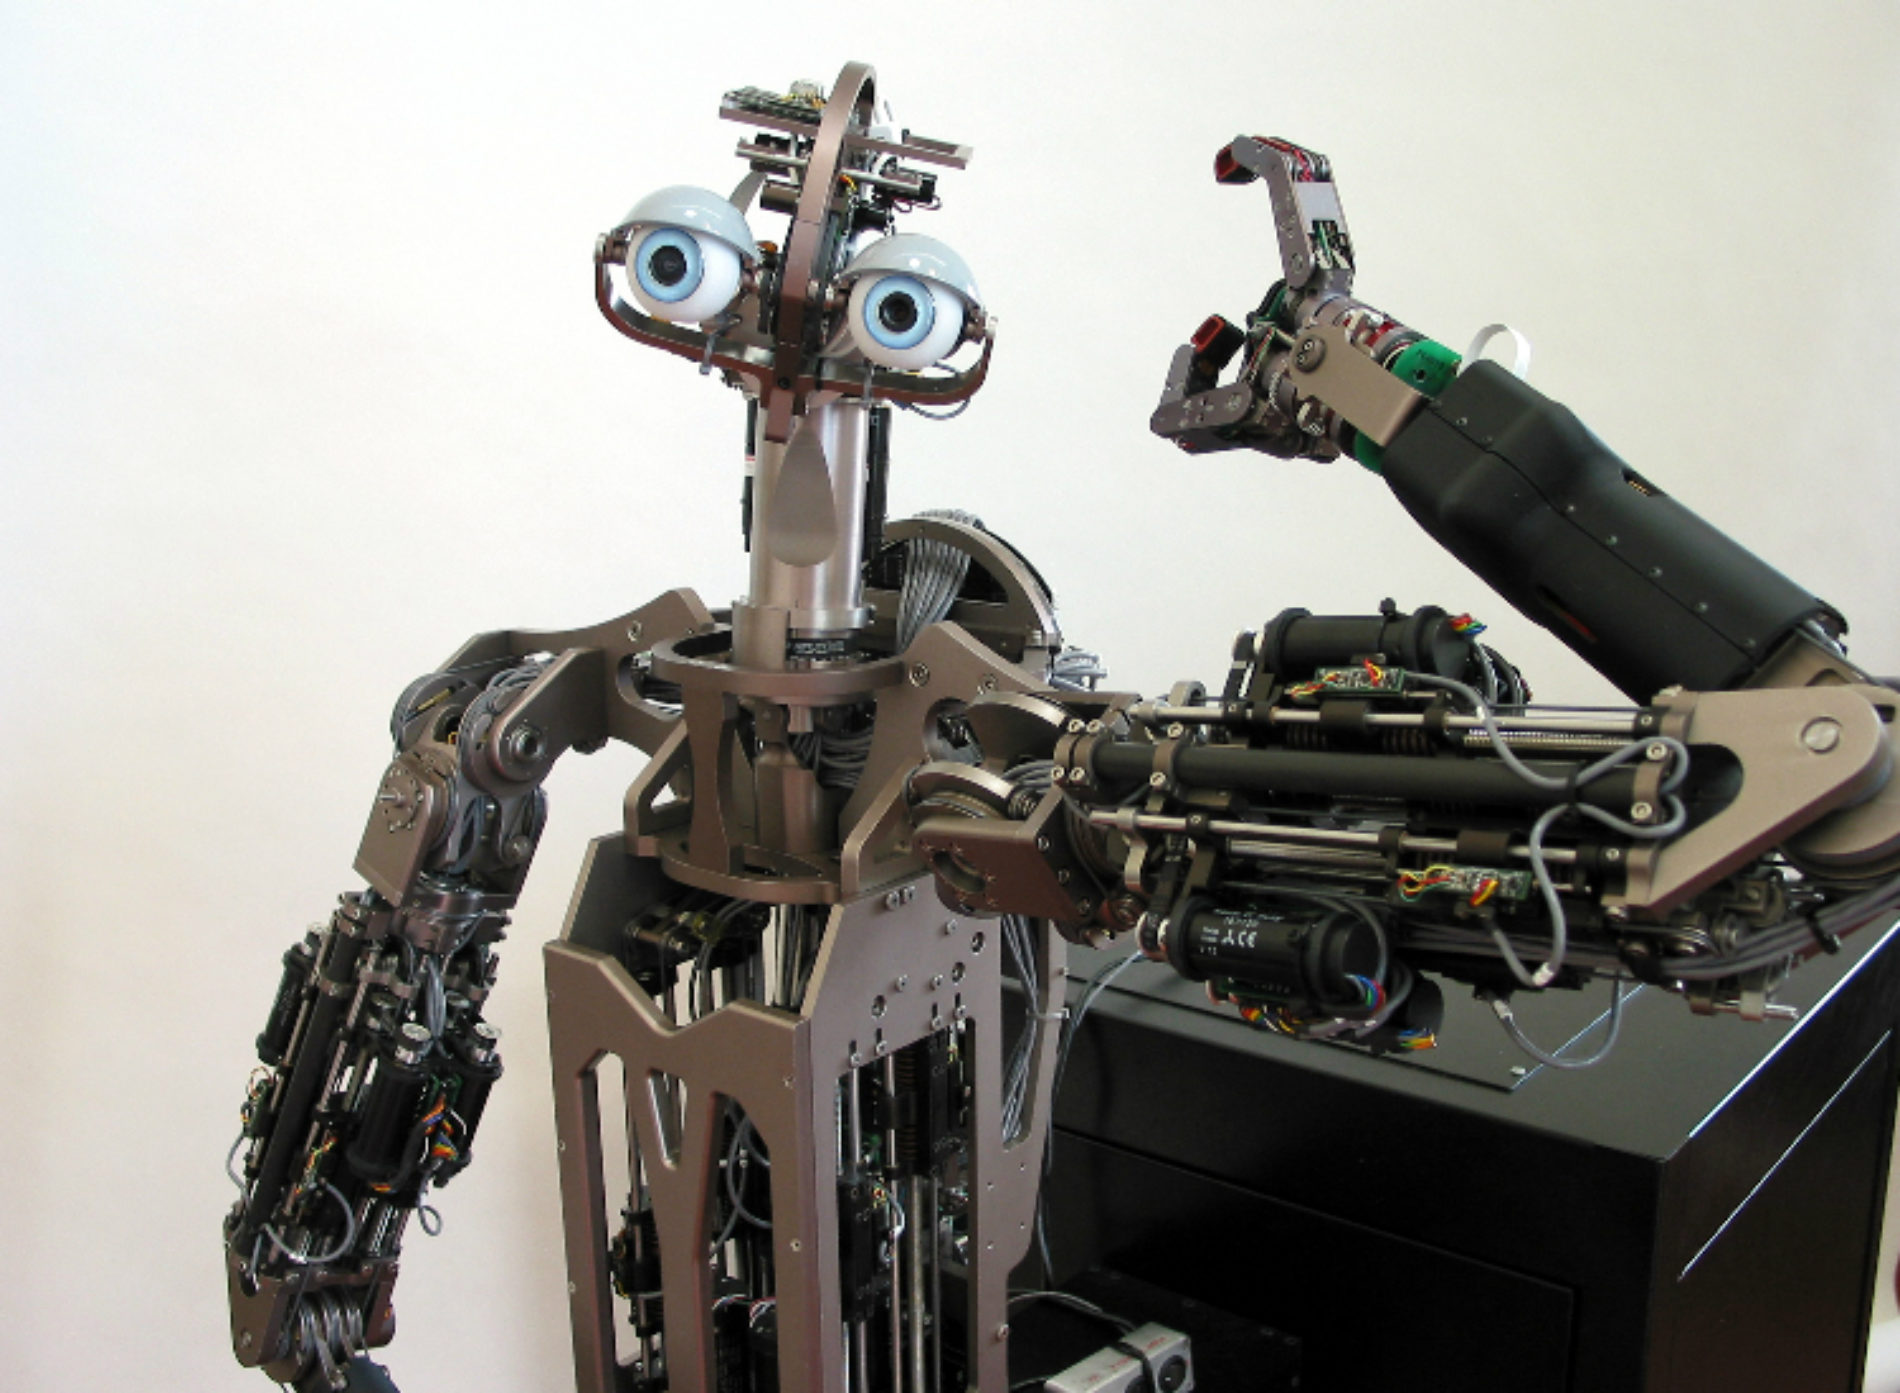
\includegraphics[width=0.6\linewidth]{tex/figs/domo-foto.jpg}
    \caption{Foto Robô Domo (Fonte: http://www.robotsvoice.com)}
    \label{fig:domorobot}
\end{figure}

Este projeto teve particular importância pois muitos dos conceitos explorados vieram a compor patentes e futuramente partes dos robôs Baxter e Meka, respectivamente das empresas Rethink Robotics e Meka Robótics. Da mesma equipe que desenvolveu o Domo surgiu a Meka Robótics a partir de Aaron Singer e Jeff Weber. E dos trabalhos de Pratt e Williason \cite{pratt1995series} surgiu a empresa Rethink Robotics fundada por Rodney Brooks, então professor do MIT em 1995.

% Baxter vs Meka
Embora com design completamente diferente, ambos robôs incorporam o uso atuadores série elásticos em cada uma das juntas como elemento de segurança. Desta forma qualquer pessoa pode manusear os braços de ambos robôs de maneira livre. No entanto este sistema também confere ao robô uma maior suscetibilidade a influência de outros estímulos externos como a ação da gravidade na dinâmica do robô tornado necessária o uso de soluções de controle complementares para garantir a precisão. \cite{nobody} Este problema é resolvido de forma diferente em cada uma das plataformas. No Baxter a compensação da gravidade é feita de forma completamente mecânica por uma série de molas \cite{nobody}, o que em parte explica seu maior tamanho. E no Meka esta é feita via software através do modelo dinâmico em conjunto da biblioteca KDL \cite{nobody}, conferindo um design mais compacto. 

% Robonauta -> Paradigmas atuais

\section{Definição do problema}

No Laboratório de Automação e Robótica ( LARA - UnB ) encontra-se disponível o braço robótico Meka A2 fornecido pela Meka Robotics. Daqui em diante será denominado apenas Meka. O Meka é um braço complacente antropomórfico composto por 7 juntas e uma garra desenvolvido para pesquisas na área de interação com pessoas. Cada uma das juntas possui um atuador série elástico composto de um motor sem escova e um redução mecânica por onda de deformação.

Em trabalhos anteriores foi observado um desempenho ineficiente nos controles cinemáticos implementados em contraste ao resultado observado em outras plataformas robóticas e em simulação. Tal arquitetura não encontra-se devidamente documentada e detalhada. Desta forma, neste trabalho, propõe-se realizar uma caracterização mais detalhada desta arquitetura de controle para compreender sua implicação no desempenho dos controles cinemáticos testados e propor melhorias que resultem em trajetórias mais precisas levando em conta as características próprias do sistema.

\section{Metodologia}

% Rever completamente
Este trabalho foi desenvolvido em três etapas: estudo sobre teoria clássica de controle de manipuladores, revisão e acompanhamento de trabalhos anteriores feitos no LARA utilizando o Meka e por fim a investigação e experimentação usando a plataforma. Esta investigação foi feita a partir da métodos científicos de análise e síntese do processo. Por meio da análise foram estudados cada um dos componentes utilizados tanto de hardware como software em seu detalhes. E contraponto foi alguns dos fenômenos foram sintetizados por meio de simulações visando ampliar a compreensão de quais fatores ocasionam ao Meka um desempenho inferior outros braços robóticos avaliados pelos trabalhos de Murilo \cite{nobody} e Marcos \cite{nobody}.

\subsection{Estudo controle de manipuladores}

Inicialmente foi feito um estudo sobre a teoria clássica do controle cinemático e dinâmico de manipuladores incluindo a representação por cadeia cinemática usando matrizes homogenias e a simplificação através da notação de Denavit-Hatemberg.

\subsection{Revisão trabalhos anteriores}

Inicialmente foi feito um estudo sobre os trabalho anteriores desenvolvidos na plataforma no Laboratório de Automação e Robótica ( LARA - UnB ) bem como estratégias clássicas no controle de robôs industriais. Alguns destes trabalhos puderam ser acompanhados ao longo da execução como o caso dos trabalhos desenvolvidos por Marcos Pereira e pelo Rafael Koji de modo a facilitar a transmissão do conhecimento relacionado as contribuições de cada um ao projeto bem como presenciar as dificuldades relacionadas ao controle do braço robótico.

\subsection{Investigação e experimentação a partir da plataforma}

Após o estudo preliminar foi adotado uma metodologia de investigação baseada em ciclos compostos por 3 etapas, descritas a seguir. Estas etapas são baseadas nos princípios de desenvolvimento ágil \ref{noref} e têm como objetivo acelerar e otimizar os esforços.

% TODO Colocar Referência

% Diagrama das etapas
\begin{enumerate}
    \item Análise e Formulação de Hipóteses
    \item Formulação de Testes para as Hipóteses
    \item Avaliação de Hipóteses ( Testes Experimentais e Estudo teórico )
\end{enumerate}

Cada ciclo possui duração variável de acordo com o nível de aprofundamento necessário para satisfazer os objetivos levantados para cada momento do projeto. O objetivo central é ao final de um ciclo é trazer algum aprimoramento quanto ao entendimento do sistema ou ainda quanto ao comportamento final na realização da tarefa.

No inicio de cada ciclo é feito um estudo do sistema através da modelagem do sistema e da definição de uma métrica para avaliar o comportamento. Então o comportamento do sistema real é comparado com o modelo adotado e as expectativas de comportamento. Os objetivos são traduzidos em uma métrica, compondo um conjunto de indicadores que permita avaliar se tarefa foi executada e como foi o processo de execução. A cada novo aspecto avaliado podem ser introduzidos novos indicadores em conjunto aos antigos ou modificados. 

Com base nisto são levantadas hipóteses quanto ao comportamento quanto ao fato de satisfazer ou não o modelo adotado e possíveis condutas para aprimorar os resultados dentro da métrica proposta. Para cada uma destas condutas é levantado um teste de verificação que pode incluir consulta bibliográfica, simulações a partir do modelo e experimentos com o Meka. Os resultados desta etapa são então levados para a etapa de observação e confrontados novamente e assim o ciclo se repete.

Resultados positivos são incorporados e resultados negativos avaliados quanto a possíveis correções. Tudo é registrado para permitir futuras avaliações. O resultado de cada dia foi feito um registro das atividades e todo material produzido foi colocado no GitHub \footnote{www.github.com/lara-unb/Meka} de forma a permitir o uso futuro na validação do comportamento após modificações futuras.

\section{Estrutura do Documento}

Este trabalho está dividido em 5 capítulos visando facilitar o entendimento. Estes estão organizados da seguinte forma:

\begin{itemize}
    \item \textit{Cap. \ref{ch:intro} Introdução} : Breve Apresentação e Histórico sobre Robótica Colaborativa.
    \item \textit{Cap. \ref{ch:teory-reference} Fundamentos} : Conceitos teóricos e tecnologias usadas no trabalho.
    \item \textit{Cap. \ref{ch:develop} Desenvolvimento} : Metodologia usada na investigação dos problemas e análise dos dados.
    \item \textit{Cap. \ref{ch:results} Resultados} : Dados obtidos ao longo do trabalho.
    \item \textit{Cap. \ref{ch:conclusoes} Conclusão} : Resultado final do trabalho e propostas de trabalhos futuros.
\end{itemize}
